%%%%%%%%%%%%%%%%%%%%%%%%%%%%%%%%%%%%%%%%%%%%%%
%\chapter{Introduction}
%%%%%%%%%%%%%%%%%%%%%%%%%%%%%%%%%%%%%%%%%%%%%%
%High energy electrons scattering on a nuclear target provides an essential probe to unveil the tiny structure of nuclei and nucleons. The electron interacts with the target by exchanging a virtual photon which includes both the longitudinal and transverse components, comparing with the transversely polarized real photon. In the kinematic region of quasi-elastic (QE) scattering, the virtual photon is able to couple to a meson which is exchanged between two nucleons. The measurement of such process is able to resolve the nucleon-nucleon (NN) interaction and provide an effective way to study the structure of nuclear as discussed in next chapter.

% In this chapter, a review of QE electron-nucleus scattering will be given, followed by a discussion of extracting the spectral function and the momentum distribution of the knock-out nucleon via the inclusive cross sections measurement.

\section{Electron-Nucleus Quasi-elastic Scattering}
\begin{figure}[!ht]
  \begin{center}         
    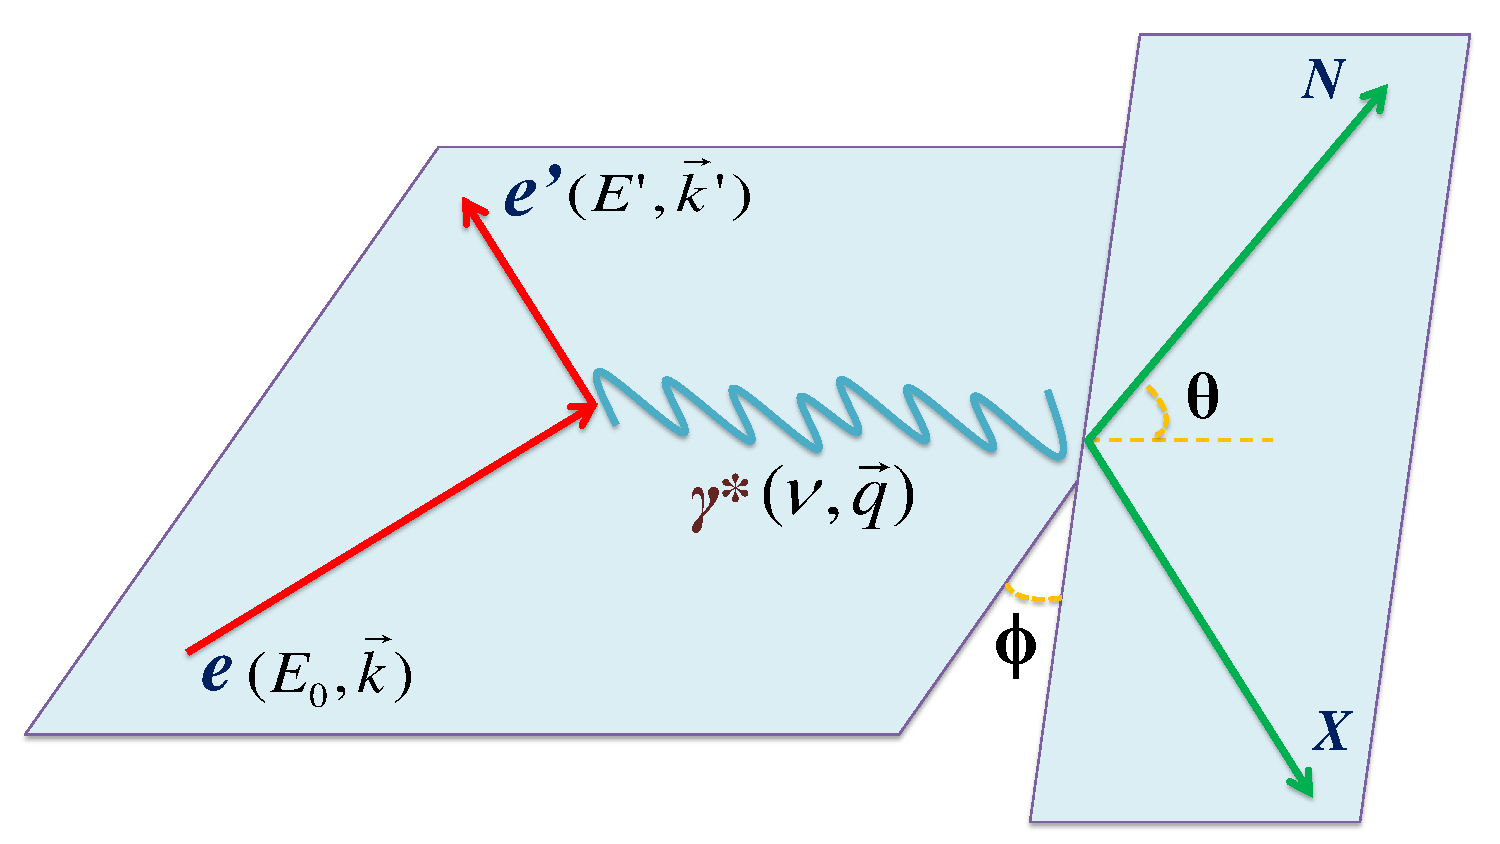
\includegraphics[type=pdf,ext=.pdf,read=.pdf,width=0.60\linewidth]{./figures/physics/e_scatt}
    \caption[Schematic of electron-scattering on a nucleus]{\footnotesize{Schematic of electron-scattering on a nucleus}}
    \label{e_scatt}
  \end{center}
\end{figure}
An electron with predefined initial energy and final energy, $E_{e}$ and $E'_{e}$, interacts with a charged nucleus by exchanging a virtual photon with the energy transfer, $\nu = E_{e}-E'_{e}$ (Fig.~\ref{e_scatt}). By varying the amplitude of the energy transfer, one can probe the nucleus at different scales. At low energy transfer, electrons interact with the entire nucleus and the measurement of elastic cross section is generally applied in the study of nuclei and nucleons form factors~\cite{bfrois}. 

As shown in Fig.~\ref{e_trans}~\cite{qe_donal}, a process of quasi-elastic (QE) electron-nucleon scattering appears with larger energy transfer, and the Fermi motion of the nucleon in the nucleus results an broad distribution compared to the shape elastic peak. Nucleons are excited at even larger energy transfer and resonances start to contribute to the cross section. 

Electrons directly probe the quarks properties at very large energy transfer through the process of deep inelastic scattering (DIS). 
\begin{figure}[!ht]
  \begin{center}
    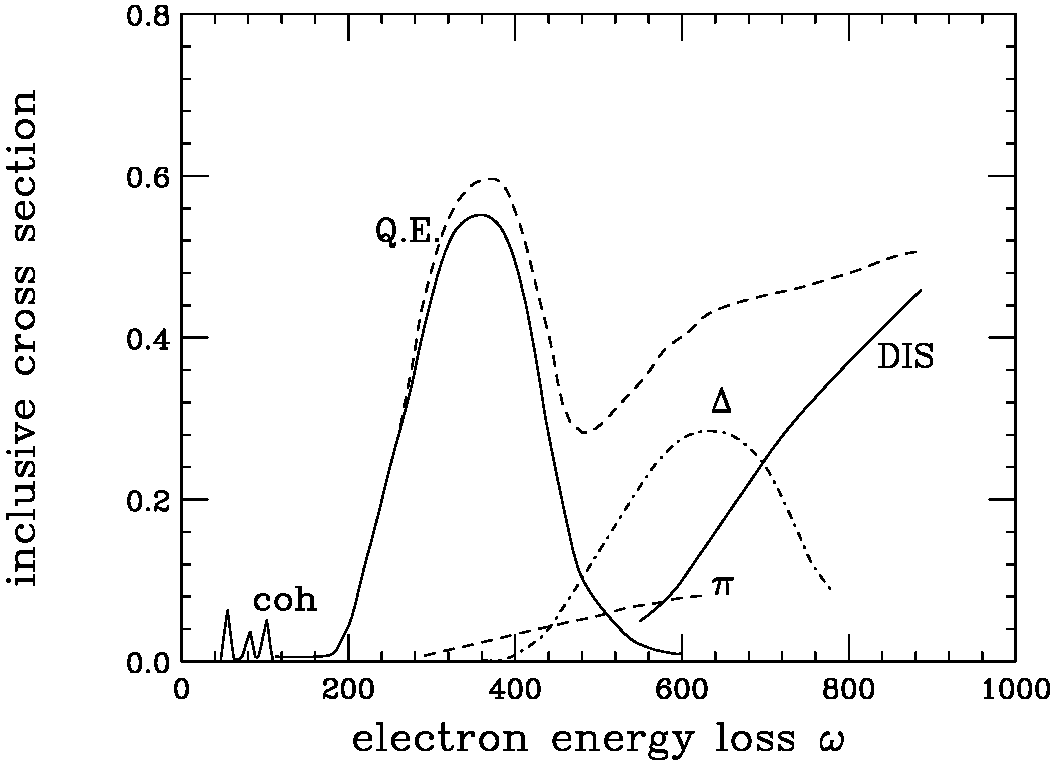
\includegraphics[type=pdf,ext=.pdf,read=.pdf,width=0.60\linewidth]{./figures/physics/eesm}
    \caption[Electron energy transfer]{\footnotesize{Inclusive cross section on the y-axis versus the energy loss,$\omega=\nu=E_{e}-E'_{e}$, on the x-axis.}}
    \label{e_trans}
  \end{center}
\end{figure}

A convenient parameter for identifying different processes in the scattering is the Bjorken variable, $x_{bj}=Q^{2}/(2m_{N}\nu)$, where $m_{N}$ is the nucleon mass. The original definition of $x_{bj}$ is the momentum fraction of the quark constituents from the nucleon during the DIS scattering. In electron-nucleon scattering, the elastic peak locates at $x_{bj}=1$, while for inelastic process, $0<x_{bj}<1$. In electron-nucleus scattering, $x_{bj}$ extends to the region of $0<x_{bj}<M_{A}/m_{N}$, $x_{bj}=1$ is now the location of the quasi-elastic peak, and the elastic peak moves to $x_{bj}=M_{A}/m_{N}$. For convenience, $m_{N}$ is usually replaced by the proton mass during the experimental data analysis, as used in the rest of this thesis:
\begin{equation}
  x_{bj} = Q^{2}/(2m_{p}\nu).
  \label{xbj_define}
\end{equation}  

During the quasi-elastic scattering, an electron knocks a nucleon out from the nucleus (Fig.~\ref{e_scatt}), which provides a opportunity to study the property of nuclear structure. In the picture of plane-wave impulse approximation (PWIA), the exclusive electron scattering cross section is the sum of the cross sections of the individual nucleons as:~\cite{john_thesis}:
\begin{equation}
  \frac{d^{5}\sigma}{dE'_{e}d\Omega_{e} d^{3}\vec{p'}} = \sum_{nucleons}\sigma_{eN}\cdot S'_{N}(E_{0},\vec{p}_{0}),
  \label{quasi_xs_spectral_function}
\end{equation}
where $S'_{N}(E_{0},\vec{p}_{0})$, called the nuclear spectral function, is the probability of removing a nucleon with initial energy $E_{0}$,  and momentum $\vec{p}_{0}$ from the target nucleus~\cite{qe_donal}, and $\sigma_{eN}$ is the electron-nucleus cross section. 

%%%%%%%%%%%%%%%%%%%%%%%%%%%%%%%%%%%%%%%%%% 	  
\subsection{Inclusive Cross Section}
%%%%%%%%%%%%%%%%%%%%%%%%%%%%%%%%%%%%%%%%%% 	  
\begin{figure}[!ht]
  \begin{center}
    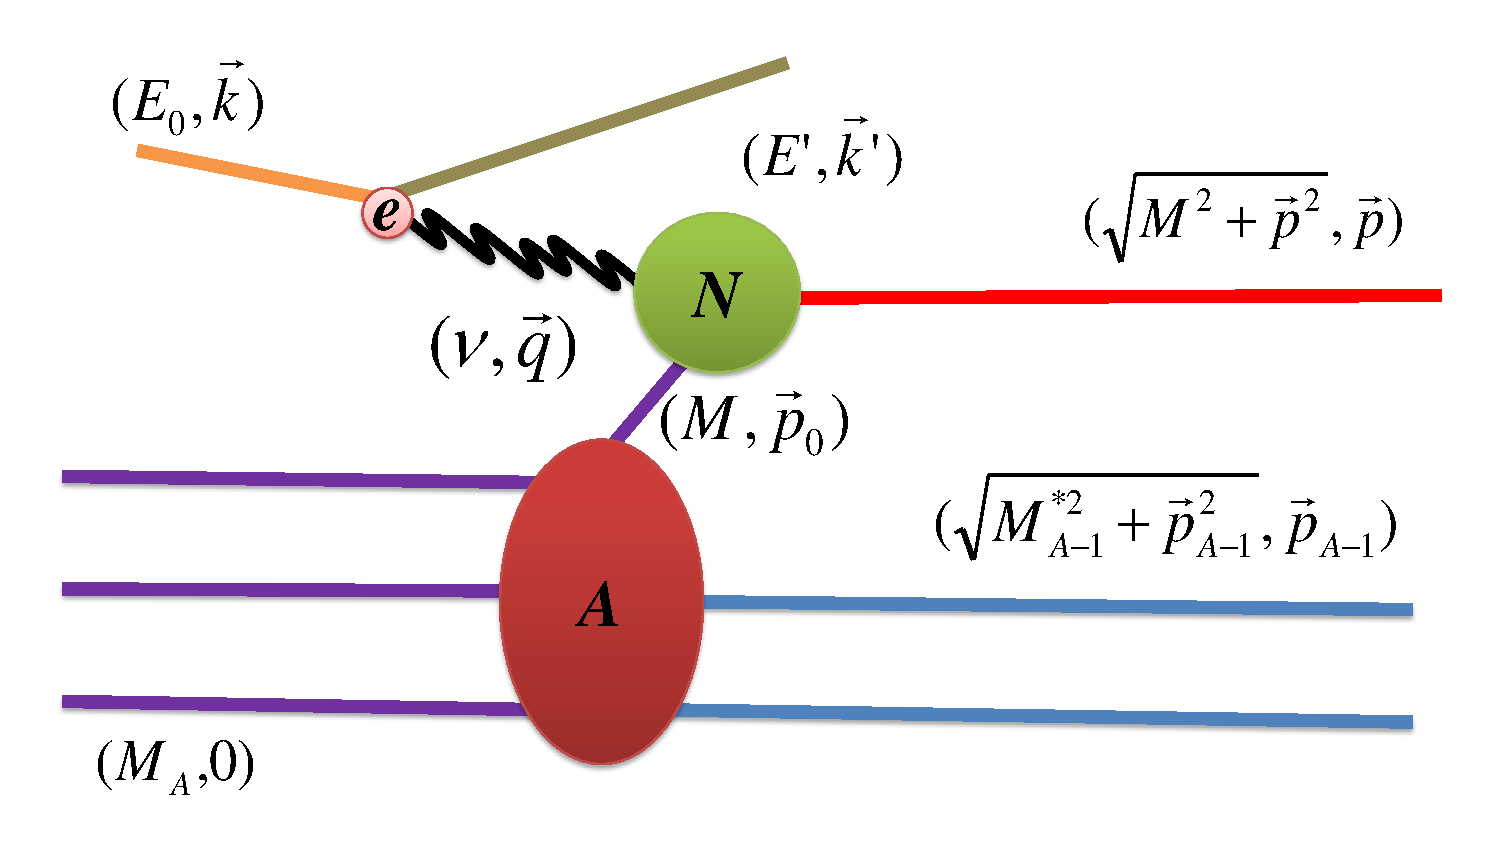
\includegraphics[type=pdf,ext=.pdf,read=.pdf,width=0.60\linewidth]{./figures/physics/includ_diagram}
    \caption[Schematic of inclusive QE electron scattering]{\footnotesize{Schematic of inclusive QE electron scattering where $\vec{p}_{A-1} = -\vec{p}_{0}$ for fixed targets.}}
    \label{includ_scatt_diag}
  \end{center}
\end{figure}
As shown in Fig.~\ref{includ_scatt_diag}, the inclusive electron scattering cross section is measured by only detecting the scattered electrons ($\sqrt{M^{2}+ \vec{p}^{2}}$, $\vec{p}$), while the final state of the ($A-1$) recoil system,($\sqrt{M_{A-1}^{2}+ \vec{p}_{A-1}^{2}}$, $\vec{p}_{A-1}$), remains unknown. To obtain the inclusive cross section from Eq~\eqref{quasi_xs_spectral_function}, one separates the contributions from protons and neutrons, and integrates over the final states of the nucleons:
\begin{equation}
  \frac{d^{3}\sigma}{dE'd\Omega} = \int (Z\sigma_{ep}S'_{p}(E_{0},\vec{p}_{0})+N\sigma_{en}S'_{n}(E_{0},\vec{p}_{0})) d^{3}\vec{p},
\end{equation}
where the subscripts in $dE'_{e}d\Omega_{e}$ have been omitted since only electrons are measured.

Assuming the spectral function is spherically symmetric, and if the difference in the spectral function between protons and neutrons is ignored, the more general form $S'(E_{0},p_{0})$ can be factored out from the equation. Since $\vec{p} = \vec{p}_{0}+\vec{q}$, where $\vec{q}$ is fixed when measuring $E_{0}$ and $E'$, one can replace $d^{3}\vec{p}$ by $d^{3}\vec{p}_{0}$. In the spherical coordinate, $d^{3}\vec{p}_{0}=p_{0}^{2} dp_{0}d(cos\theta) d\phi$, and the cross section becomes:
\begin{equation}
  \frac{d^{3}\sigma}{dE'd\Omega} = 2\pi \int \tilde{\sigma}_{0}\cdot S'(E_{0},p_{0})\cdot p_{0}^{2}dp_{0}d(cos\theta)
  \label{in_xs_org}
\end{equation}
where
\begin{equation}
  \tilde{\sigma}_{0} = \frac{1}{2\pi}\int_{0}^{2\pi} \left( Z\sigma_{ep}+N\sigma_{en} \right)d\phi.
\end{equation}

Eq~\eqref{in_xs_org} can be further simplified by considering the energy conservation. From Fig.~\ref{includ_scatt_diag}, for the fixed target, $\vec{p}_{A-1} = - \vec{p}_{0}$, which gives: 
\begin{equation}
  M_{A}= E_{0}+ \sqrt{M_{A-1}^{*2}+p_{0}^{2}},
\end{equation}
and,
\begin{equation}
  \quad  M_{A}+\nu = \sqrt{M^{2}+(\vec{p}_{0}^{2}+\vec{q}^{2})}+\sqrt{M_{A-1}^{*2}+\vec{p}_{0}^{2}},
  \label{ene_mom_cons}
\end{equation}
where $M$, and $M_{A}$ are the mass of the ejected nucleon and the target nucleus, respectively. $M_{A-1}^{*}$ is the mass of the recoiling $(A-1)$ system, where the superscript * means it could be in its excited state. Eq~\ref{in_xs_org} becomes~\cite{john_thesis}:
\begin{equation}
  \frac{d^{3}\sigma}{dE'd\Omega} = 2\pi \int \tilde{\sigma}_{0}\cdot \frac{E_{N}}{|\vec{p}_{0}||\vec{q}|} \cdot S'(E_{0},p_{0})\cdot p_{0}^{2}dp_{0}dE_{0}
\end{equation}
where $E_{N}=\sqrt{M^{2}+\vec{p}}$ denotes the energy of the struck nucleon.

One can define the separation energy, $E_{s}\equiv M_{A-1}^{*}+M-M_{A}$. Then the spectral function becomes $S(E_{s},p_{0})\equiv - S'(E_{0},p_{0})$, where the Jacobian transformation factor from $E_{0}$ to $E_{s}$ has been absorbed into the new definition~\cite{john_thesis}. One can define $\tilde{\sigma}=\tilde{\sigma_{0}}\cdot E_{N}/|\vec{q}|$, and rewrite the cross section as:
\begin{equation}
  \frac{d^{3}\sigma}{dE'd\Omega} = 2\pi \int_{E_{s}^{min}}^{E_{s}^{max}} \int_{p_{0}^{min}}^{p_{0}^{max}}\tilde{\sigma}\cdot S(E_{s},p_{0})\cdot p_{0}dp_{0}dE_{s},
  \label{in_qe_xs1}
\end{equation}
where $p_{0}^{min}$ and $p_{0}^{max}$ are the solution of Eq~\eqref{ene_mom_cons} when $\vec{p}_{0}$ and $\vec{q}$ are parallel:
\begin{equation}
  \quad  M_{A}+\nu = \sqrt{M^{2}+y^{2}+2yq+q^{2}}+\sqrt{M_{A-1}^{*2}+y^{2}},
  \label{ene_mom_cons_y}
\end{equation}	
where two solutions, $y_{1}$ and $y_{2}$ ($y_{1}<y_{2}$), give the values of $p_{0}^{min}$ and $p_{0}^{max}$, respectively. While $E_{s}^{min}$ corresponds to the minimum separation energy when the recoil nucleus is in its ground state, $E_{s}^{max}$ is the maximum separation energy when the struck nucleon is at rest:
\begin{equation}
  E_{s}^{max}=\sqrt{(M_{A}+\nu)^{2}-q^{2}}-M_{A}.
\end{equation}
which leads to $p_{0}^{min}(E_{s}^{max}) = p_{0}^{max}(E_{s}^{max})$.

\begin{figure}[!ht]
  \begin{center}
    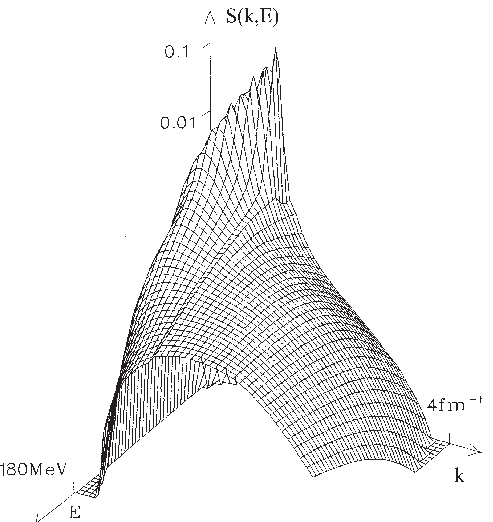
\includegraphics[type=pdf,ext=.pdf,read=.pdf,width=0.60\linewidth]{./figures/physics/pkem}
    \caption[Spectral Function]{\footnotesize{Spectral Function versus separation energy $E_{s}$ and transfer momentum $p_{0}$~\cite{qe_donal}.}}
    \label{pkem}
  \end{center}
\end{figure}
Because the spectral function decreases rapidly by orders of magnitude toward $E_{s}^{max}$ and $p_{0}^{max}$, see Fig.~\ref{pkem}, the upper limits of the two integrals in Eq~\eqref{in_qe_xs1} can be extended to infinity. Meanwhile, $\tilde{\sigma}$ changes very slow as a function of $E_{s}$ and $p_{0}$ so can be factored out from the integral and evaluated at the maximum value of the spectral function at $E_{s}=E_{s}^{0}$. Hence Eq~\eqref{in_qe_xs1} can be rewritten as:
\begin{equation}
  \frac{d^{3}\sigma}{dE'd\Omega} = 2\pi \bar{\sigma}\int_{E_{s}^{min}}^{\infty} \int_{p_{0}^{min}}^{\infty}S(E_{s},p_{0})\cdot p_{0}dp_{0}dE_{s},
  \label{in_qe_xs2}
\end{equation}
where $\bar{\sigma} \propto \tilde{\sigma}(E_{s}^{0},p_{0}^{min})$~\cite{PhysRevB.36.1208}. The model of $\bar{\sigma}$ is usually taken from the prescription by De Forest~\cite{DeForest1983}, shown as~\cite{john_thesis}:
\begin{equation}
  \bar{\sigma} = \frac{1}{Z\sigma_{p}+N\sigma_{n}}\frac{|\vec{q}|}{\sqrt{M^{2}+(y+\vec{q})^{2}}}.
\end{equation}

%%%%%%%%%%%%%%%%%%%%%%%%%%%%%%%%%%%%%%%%%%%%%%%%%%%%%%%%%%%%%%%%%%%
\subsection{Momentum Distribution and y-Scaling}
%%%%%%%%%%%%%%%%%%%%%%%%%%%%%%%%%%%%%%%%%%%%%%%%%%%%%%%%%%%%%%%%%%% 	  
The integral of the spectral function over the separation energy leads to the momentum distribution:
\begin{equation}
  n(p_{0}) = \int_{E_{s}^{min}}^{\infty} S(E_{s},p_{0})dE_{s},
  \label{np_mom_eq}
\end{equation}
which is a sensitive probe to examine the effect of the nuclear medium and nucleon-nucleon interactions. At momenta above the Fermi momentum, $k_{F}$, the mean field effect vanishes and strong short range correlations of the nucleons emerge.

The spectral function is directly connected to the momentum distribution, but it is not an experimental observable. Instead, one can examine the scaling behavior~\cite{West1975263} of inclusive quasielastic scattering cross section. The scaling function can be defined as~\cite{PhysRevC.41.R2474,Boffi19931}:
\begin{equation}
  F(y,q) = 2\pi\int_{E_{s}^{min}}^{\infty} \int_{|y|}^{\infty}S(E_{s},p_{0})\cdot p_{0}dp_{0}dE_{s}.
  \label{fy_scaling_eq}
\end{equation}
where the new variable, $y$, is defined as the minimum values of momentum in Eq~\eqref{ene_mom_cons}, $p_{0}^{min}=|y|$, when the $A-1$ system is in its ground state:
\begin{equation}
  M_{A}+\nu = \sqrt{M^{2}+q^{2}+y^{2}+2yq}+\sqrt{M_{A-1}^{2}+y^{2}}.
  \label{y_enegy_conserv}
\end{equation} 
If only the nucleonic degrees of freedom are considered, the scaling function becomes independent of $\vec{q}$ at large momentum transfer~\cite{Boffi19931}. Hence, $F(y,q)\equiv F(y)$. From Eq~\eqref{in_qe_xs2}, the scaling function can be extracted from electron-nucleon scattering cross section for an off-shell nucleon:
\begin{equation}
  F(y)=\frac{d^{3}\sigma}{dE' d\Omega } \frac{1}{Z\sigma_{p}+N\sigma_{n}} \frac{q}{\sqrt{M^{2}+(y+q)^{2}}}.
  \label{fy_scaling_eq2}
\end{equation}
Due to the Fermi motion, the broad quasielastic peak of the inclusive cross section is mixed with the tails of resonance and DIS components, as shown in Fig.~\ref{e_trans}. To extract $F(y)$ from the experimental cross section, one needs to utilize a cross section model to remove the contribution from DIS region, $\sigma_{QE}=\sigma_{Exp}-\sigma_{DIS}^{model}$ (See Appendix B).

By reversing the order of the integration in Eq~\ref{fy_scaling_eq} and based on Eq~\eqref{np_mom_eq}, $F(y)$ can be rewritten as:
\begin{equation}
  F(y) = 2\pi\int_{|y|}^{\infty}n(p_{0})\cdot p_{0}dp_{0}.
  \label{fy_mom_eq}
\end{equation} 
Hence the momentum distribution can be extracted experimentally by measuring the $F(y)$ distribution~\cite{qe_donal}:
\begin{equation}
  n(p_{0}) = \frac{-1}{2\pi p_{0}}\frac{dF(p_{0})}{dp_{0}} \mid_{p_{0}=|y|},
  \label{mom_dis_fy}
\end{equation}
The scaling of $F(y)$ is supposed to be valid in the limit of very large momentum transfer where the effects due to final-state interactions and the error made by extending the upper limit of Eq~\eqref{fy_mom_eq} to infinity can be neglected. Meanwhile, the assumption that the lower limit ($p_{0}^{min}=|y|$) is independent of $E_{s}$ is also needed to be verified. The momentum distribution can be extracted from data in the scaling region, but the data in the region of approaching to scaling is also important to verify those assumptions.
